\documentclass{standalone}
% font set
\usepackage{ctex}
\usepackage{fontspec}
\usepackage[T1]{fontenc}
\usepackage[sc]{mathpazo}
\usepackage{anyfontsize}
\setmainfont{Source Serif 4}
\setsansfont{Source Sans 3}
\setmonofont{Menlo}
\setCJKmainfont[BoldFont=黑体-简 中等,ItalicFont=楷体-简 常规体]{宋体-简 常规体}

% colors
\usepackage[dvipsnames]{xcolor}
\definecolor{pku-red}{RGB}{139,0,18}
\usepackage{colortbl}
\newcommand{\light}[1]{\textcolor{Orchid}{#1}}
\newcommand{\contrastlight}[1]{\textcolor{TealBlue}{#1}}

% plots
\usepackage{tikz}
\usepackage{tikz-cd}
\usetikzlibrary{arrows}
\usetikzlibrary{arrows.meta,positioning,calc,3d}
\usepackage{pgfplots}
\pgfplotsset{compat=newest}
\tikzset{
    punkt/.style={
        rectangle,
        rounded corners,
        draw=black, very thick,
        minimum height=2em,
        inner sep=6pt,
        text centered,
        fill=gray!30
    }
}

% math package
\let\Bbbk\relax
\usepackage{amsmath}
\usepackage{mathrsfs}
\usepackage{amssymb}
\usepackage{amsfonts}
\usepackage{stmaryrd}
\usepackage{latexsym}
\usepackage{extarrows}
\SetSymbolFont{stmry}{bold}{U}{stmry}{m}{n}

\begin{document}
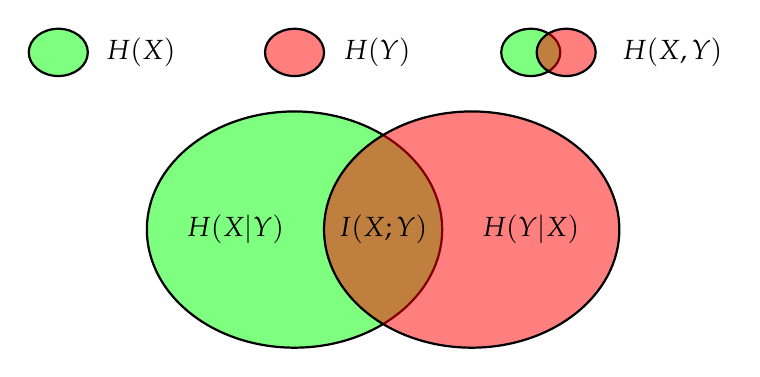
\begin{tikzpicture}[thick, scale=1.5]
    \draw [fill opacity=0.5,fill=green] (1,1) ellipse (1.25 and 1);
    \draw [fill opacity=0.5,fill=red] (2.5,1) ellipse (1.25 and 1);
    
    \draw [fill opacity=0.5,fill=green] (-1,2.5) ellipse (1.25*0.2 and 1*0.2);
    \node at (-0.3,2.5) {$H(X)$};

    \draw [fill opacity=0.5,fill=red] (-1+2,2.5) ellipse (1.25*0.2 and 1*0.2);
    \node at (-0.3+2,2.5) {$H(Y)$};

    \draw [fill opacity=0.5,fill=green] (-1+4,2.5) ellipse (1.25*0.2 and 1*0.2);
    \draw [fill opacity=0.5,fill=red] (-1+4+1.5*0.2,2.5) ellipse (1.25*0.2 and 1*0.2);
    \node at (0.2+4,2.5) {$H(X,Y)$};

    \node at (1.75,1) {$I(X;Y)$};
    \node at (0.5,1) {$H(X|Y)$};
    \node at (3,1) {$H(Y|X)$};
\end{tikzpicture}
\end{document}